\section{Perils of disregard}
\label{sec:graph-importance}

As stated in Section \ref{sec:intro}, transportation demand models are used to evaluate the impact of policies on a certain
transportation demand related outcome. As an example, consider the proposals from the following fictitious scenarios:
\begin{itemize}
 \item Based on input from the public, the Department of Transportation (DOT) is considering implementing a new parking policy.
 This proposed policy would change prices and restrict availability to discourage individuals from parking in the central business district.
 The DOT and its constituents believe that this policy will encourage people to use more active transportation modes (e.g., walking, biking, etc.) and cause them to drive less.
 \item A certain DOT is considering constructing a streetcar (trolley, tram) line in a low/mid-income area in its jurisdiction.
 Citing examples from other cities and countries, the DOT claims that the new streetcar line will create more transit oriented developments and increase economic activity in the areas surrounding the proposed project.
 \end{itemize}

%% TODO: Present an example or two of real life project proposals?

Thinking more closely about these proposals, it is clear that they assume a causal relationship between the proposed project/policy and the desired goals.
The DOT in question analyzed data, concluding that such a policy or project would cause the desired output and achieve the desired goal.
In the presented scenarios, the DOT claims that implementing the new parking policy will cause an increase the share of
active transportation modes in the central business district and that constructing the proposed streetcar line will
cause more transit oriented developments and economic activity.

Policymakers base their analyses and conclusions on hypotheses or beliefs of how the world operates.
In other words, the data analysis is based on specific beliefs about the data generating process.
However, policymakers often do not present these beliefs in a clear and concise manner.
As a result, these proposals maintain an obscure representation of how the policy or project will achieve their desired goals.

DAGs allow one to clearly encode their assumptions about the data generating process and the problem at hand.
Researchers and practitioners have made use of DAGs in fields ranging from medicine and epidemiology (\citet{shrier_2008_reducing, sung_2012_reducing}) to economics (\citet{white_2011_covariate}) and have found them to be practical.

Likewise, DAGs could prove useful in addressing transportation policy questions.
\citet{brathwaite_2018_causal} have proposed a framework illustrating how practitioners and researchers can use DAGs to answer such transportation modelling questions in a causal context.
However, \citet{brathwaite_2018_causal} did not show an empirical application of their framework and how it results in different conclusions when compared to traditional modelling approaches.

In this section, we will present an example illustrating the importance of using DAGs in transportation demand modelling.
Specifically, we will illustrate how different assumptions about the data generating process result in different conclusions, even while assuming the same outcome model.
To make our point, we build upon \citet{brathwaite_2018_causal}.
Here, we present an empirical exercise using a simplified transportation modelling problem.
Before going any further, we note that this example is illustrative, and it does not reflect all complexities in a typical transportation choice modelling problem.
Indeed, it is not our primary goal in this section to recover the causal effect of the proposed intervention.
Instead, we are most interested in showing how different DAGs would result in different conclusions about the effect of the proposed intervention.

Let us assume that a company wants to reduce its workforce carbon footprint by moving its employees closer to their campus.
We would like to forecast how such an intervention would change the share of employees driving to work.
We model this travel mode choice problem based on a dataset from \citet{brathwaite_asymmetric}.
This dataset is based on the 2012 California Household Travel Survey, and it
contains approximately 4000 home-based school or work tours made by approximately 3850 individuals in the California Bay area.
The dataset includes eight travel modes. 
For our illustrative purposes, we focus on the following car-centric modes:

\begin{itemize}
   \item Drive Alone: The individual uses a private vehicle to make the trip
   \item Shared Ride 2: The individual shares an automobile ride with one more individual
   \item Shared Ride 3+: The individual shares an automobile ride with two or more individuals
\end{itemize}

Readers interested in a more detailed description of the dataset can refer to \citet{brathwaite_asymmetric}.
For the purposes of this exercise, we treat the multinomial logit model (MNL) defined in \citet{brathwaite_asymmetric} as the true outcome generating model.

In this model, the systematic utility equations of the car-centric modes defined above are specified as follows:
\begin{equation}
   \begin{aligned}
   \textrm{Utility} \left(\textrm{Drive Alone}\right) &= \beta_{\textrm{travel\_time}} \times \textrm{Travel\_Time} + \beta_{\textrm{cost\_per\_distance\_drive\_alone}} \times \textrm{Cost\_per\_Distance}_{\textrm{da}} \\
   &\quad + \beta_{\textrm{autos}} \times \textrm{Number\_of\_Autos} \\
   \textrm{Utility} \left(\textrm{Shared Ride 2}\right) &= ASC_{\textrm{shared\_ride\_2}} + \beta_{\textrm{time\_drive}} \times \textrm{Travel\_Time} \\
   &\quad + \beta_{\textrm{cost\_per\_distance\_shared\_ride\_2}} \times \textrm{Cost\_per\_Distance}_{ \textrm{sr2} } + \beta_{\textrm{autos}}  \times \textrm{Number\_of\_Autos} \\
   &\quad + \beta_{\textrm{cross\_bay}} \times \textrm{Cross\_Bay} + \beta_{\textrm{hh\_size}} \times \textrm{Household\_Size} \\
   &\quad + \beta_{\textrm{n\_kids\_hh}} \times \textrm{Number\_of\_kids} \\
   \textrm{Utility} \left(\textrm{Shared Ride 3+}\right) &= ASC_{\textrm{sr3+}} + \beta_{\textrm{time\_drive}} \times \textrm{Travel\_Time} \\
   &\quad + \beta_{\textrm{cost\_per\_distance\_sr3+}} \times \textrm{Cost\_per\_Distance}_{\textrm{sr3+}} + \beta_{\textrm{autos}}  \times \textrm{Number\_of\_Autos} \\
   &\quad + \beta_{\textrm{cross\_bay}} \times \textrm{Cross\_Bay} + \beta_{\textrm{hh\_size}} \times \textrm{Household\_Size} \\
   &\quad + \beta_{\textrm{n\_kids\_hh}} \times \textrm{Number\_of\_kids} \\
   \end{aligned}
\end{equation*}

Note that, since we consider this model to be the true outcome model, there are no latent variables we need to account for.
Below is a description of the key variables included in the model:

\begin{itemize}
  \item Total Travel Distance: the total travel distance for individual i and mode j, for all available modes for individual i during trip t of tour l.
  \item Total Travel Cost: the travel cost in dollars for individual i and mode j, for all available modes for individual i during trip t of tour l.
  \item Total travel time: the travel time in minutes for individual i and mode j, for all available modes for individual i during trip t tour l.
  \item Number of Autos: the number of automobiles owned by individual i's household.
  \item Number of Licensed Drivers: is the number of licensed drives in individual i's household.
  \item Number of Kids: the number of kids in individual i's household.
  \item Cross-bay trip: a binary variable indicating whether the trip t in tour l for individual i is a cross-bay trip.
\end{itemize}

Figure \ref{fig:IND_GRAPH} illustrates the DAG where all explanatory variables in each utility equation are marginally independent.
This DAG is equivalent to what an analyst assumes when they only update the variables directly impacted by a given policy, without considering the dependencies between the explanatory variables. 
To illustrate the problem with this approach, consider the case where the ``true'' data generating process that reflects the dependencies between the covariates is as shown in Figures \ref{fig:DA_causal_2} through \ref{fig:SR3_causal_2}. 
Under this generative model, intervening on one variable would also result in changes to other variables that are dependent on it.
The goal of our simulation exercise is to show that ignoring the true generative model of the data (Figures \ref{fig:DA_causal_2} through \ref{fig:SR3_causal_2}) can result in arbitrarily biased treatment effects, even if the analyst knows the true outcome model (Equations \ref{eq:DA} through \ref{eq:SR3}).

\begin{figure}
   \centering
   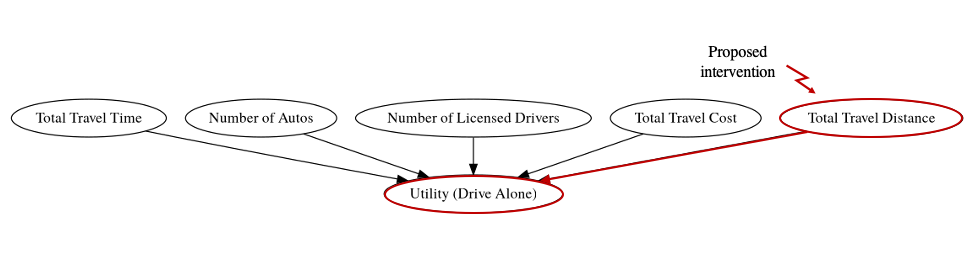
\includegraphics[width=0.75\textwidth]{Independent_graph}
   \caption{Causal Graph with Independent Covariates}
   \label{fig:IND_GRAPH}
\end{figure}

\begin{figure}
   \centering
   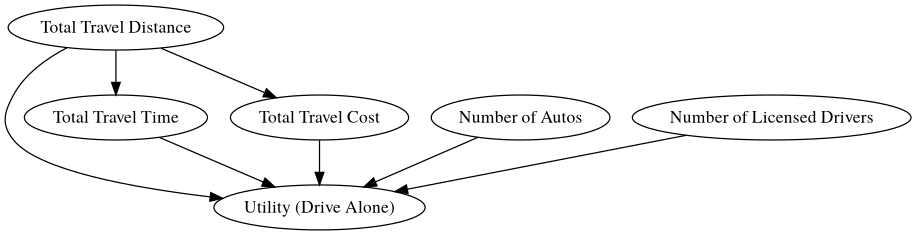
\includegraphics[width=0.75\textwidth]{DA_interacting_graph}
   \caption{Causal Graph for the Drive Alone Utility Function}
   \label{fig:DA_causal_2}
\end{figure}

\begin{figure}
   \centering
   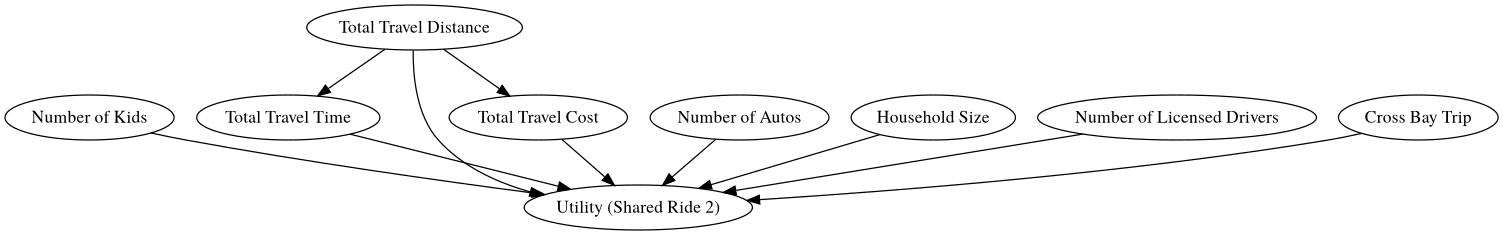
\includegraphics[width=0.75\textwidth]{SR2_interacting_graph}
   \caption{Causal Graph for the Shared Ride 2 Utility Function}
   \label{fig:SR2_causal_2}
\end{figure}

\begin{figure}
   \centering
   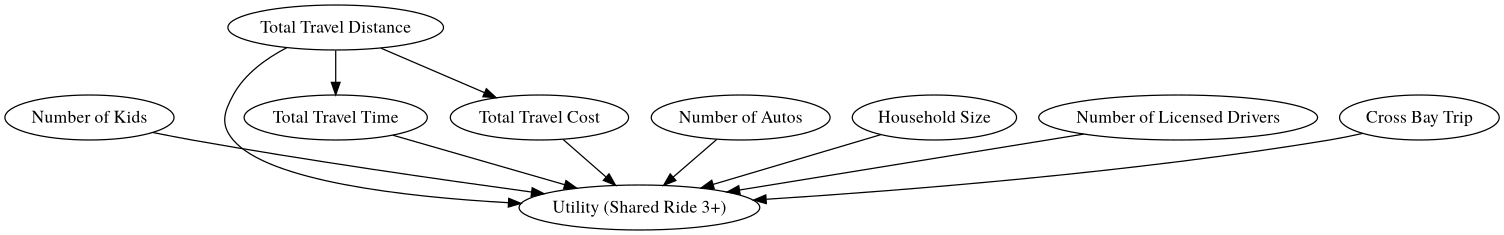
\includegraphics[width=0.75\textwidth]{SR3_interacting_graph}
   \caption{Causal Graph for the Shared Ride 3+ Utility Function}
   \label{fig:SR3_causal_2}
\end{figure}

To achieve this goal, we follow these simulation steps, using the same outcome model defined in Equations \ref{eq:DA} to \ref{eq:SR3}:
\begin{itemize}
   \item Simulate data from the DAGs shown in Figure \ref{fig:IND_GRAPH} through Figure \ref{fig:SR3_causal_2}.
   \item In one scenario, only modify the travel distance variable in all graphs to emulate a company's decision to move its employees closer to campus. This is similar to assuming the DAG in Figure \ref{fig:IND_GRAPH} as the true data generating model.
   \item In the other scenario, modify the travel distance variable in all utility graphs, as well as all the variables that are dependent on it based on the DAGs in Figure \ref{fig:DA_causal_2} through Figure \ref{fig:SR3_causal_2}. This case is meant to reflect the ``correct'' approach needed to quantify the effects of the company's policy. 
   \item Predict the probabilities of choosing car-centric modes before and after modifying the data to emulate the proposed intervention under each of the two scenarios above, and compute the differences in mode choice probabilities.
\end{itemize}

Readers interested in exploring the details of our simulation exercise can refer to our GitHub repository \citep{brathwaite_etal_2020}.


We then plot histograms of the computed differences between the average probability of an individual
in our sample choosing a car centric mode before and after implementing a policy or intervention
aimed at reducing travel distance.
Recall that these differences are plotted under the assumptions that the outcome model is the same in both scenarios, and the only difference between the two scenarios is the set of variables assumed to be affected by the proposed intervention.
This difference in the set of variables affected by the proposed intervention is a result of the two different causal graphs representing each scenario (Figures \ref{fig:IND_GRAPH} - \ref{fig:SR3_causal_2}).
Figure \ref{fig:histogram_probability} highlights the resulting bias between the estimated probability of an average individual choosing a car centric mode.
The histograms show that the distribution of inferred treatment effects based on the ``true'' causal graph includes both positive and negative treatment effects.
With low but non-trivial probability, using the wrong causal graph in one's analyses could result in not only wrong magnitudes of the treatment effect of interest but also the wrong sign.
This plotted discrepancy shows the importance of using causal graphs in the estimation of treatment effects.
Of course, the importance of a correct causal graph does not and should not take away from the importance of correctly specified outcome choice models.

\begin{figure}[h!]
   \centering
   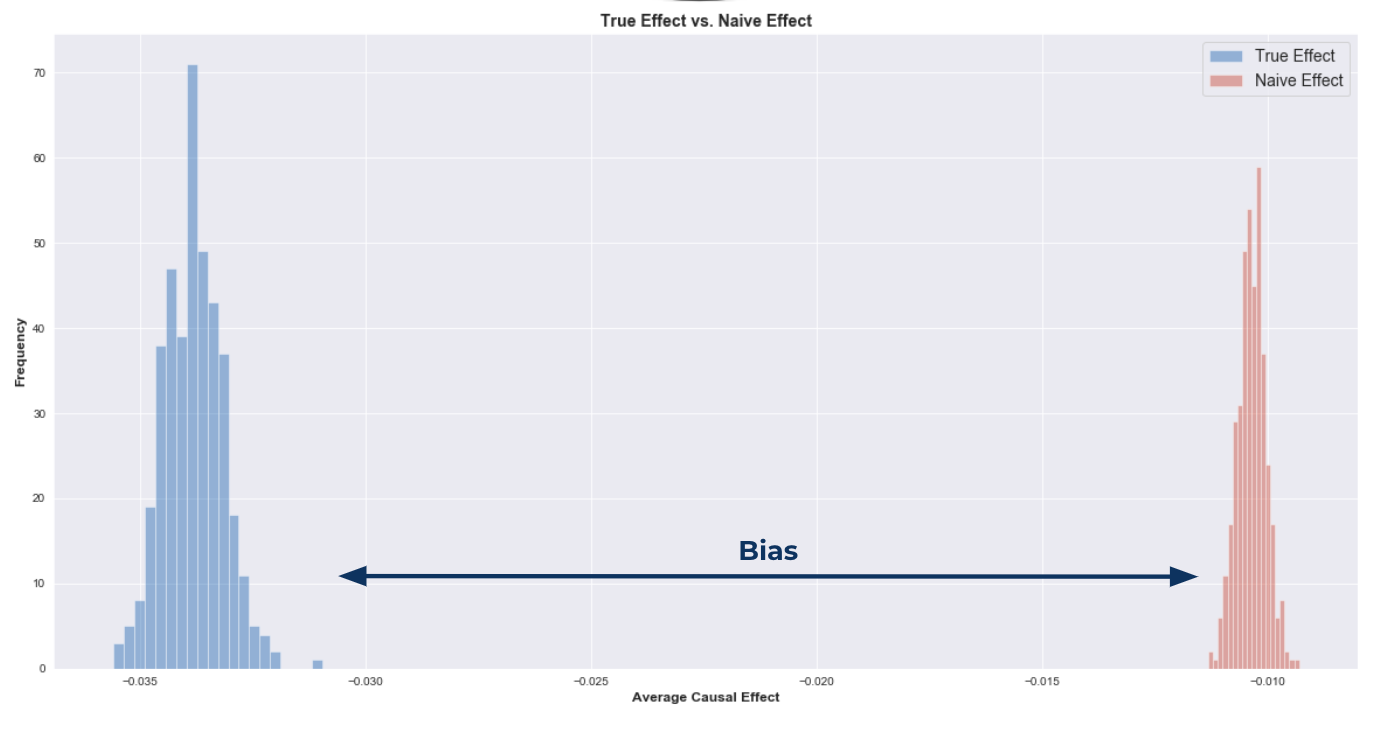
\includegraphics[width=0.95\textwidth]{histogram_selection_on_obs}
   \caption{Histograms of the probability of choosing Car Centric Modes under Different Data Generating processes.}
   \label{fig:histogram_probability}
\end{figure}

We have shown in this simulation exercise how causal graphs can be helpful in avoiding biased causal effect inferences.
Specifically, two situations highlight this fact; having mediating or confounding variables relative to the variable being intervened on in our outcome model.
In the case of mediating variables relative to the node the treatment intervenes on, we need to be careful about constructing our treatment effect estimator.
In particular, we need to ensure that we appropriately use total effect estimators instead of natural direct effect estimators.
Enacting a certain treatment shows its effect through the mediating variable.
Therefore, when ``changing'' the value of the intervention node, we need to make sure the values and distributions of any downstream nodes reflect this change.
For more information on mediating mechanisms, please refer to work by \citet{pearl_2012_mediation} and references therein.
In the case of confounding variables, we need to consider the treatment assignment mechanism when building choice models.
As \citep{hahn_2020_bayesian} show, one way to account for the treatment assignment mechanism is to estimate the propensity score in our sample and adjust for that in our outcome model.

In contrast to the example shown in this section, the data generating process might not be easily distinguishable in the majority of situations, mainly due to the complexity of the real world.
Therefore, constructing a causal graph that represents the data generating process as much as possible is not an easy task.
To prepare readers to create causal graphs, the next section will provide a brief overview of them and their history in choice modelling.
Then, Section \ref{sec:graph-construction} explores this topic and includes detailed guidance on how to build causal graphs representing the researchers beliefs about the data generating process.
Section \ref{sec:graph-testing} follows up with guidance on how to test one's causal graphs against one's data.
